% Report 6 contribution: Nguyen Lu Nhat Huy (CE181196).
% Match the common Report6 preamble; no additional packages required.
\newpage
\subsection{Contract Reviews, Banner Management and Approval Workflows}

\subsubsection{M11.05 -- Write, Update and Delete Contract Reviews}
\begin{itemize}[leftmargin=1.5em,itemsep=2pt]
  \item \textbf{Screen Name \& Route Path:}\newline \texttt{/client/reviews or /freelancer/profile?tab=reviews}.
  \item \textbf{Target Actor:} Contract participant (Client or Freelancer).
  \item \textbf{Preconditions:} Signed in; participant of an eligible completed contract; required action permission is granted.
  \item \textbf{Purpose:} Provide feedback about the other contract participant.
\end{itemize}
\paragraph{Screen-Transition Workflow:} Reviews $\rightarrow$ completed contract $\rightarrow$ review editor $\rightarrow$ submit, edit or delete confirmation.
\begin{figure}[H]\centering
\scalebox{0.20243}{%
\begingroup\setlength{\unitlength}{1pt}\linethickness{0.9pt}
\begin{picture}(450.00,479.78)
\put(0,0){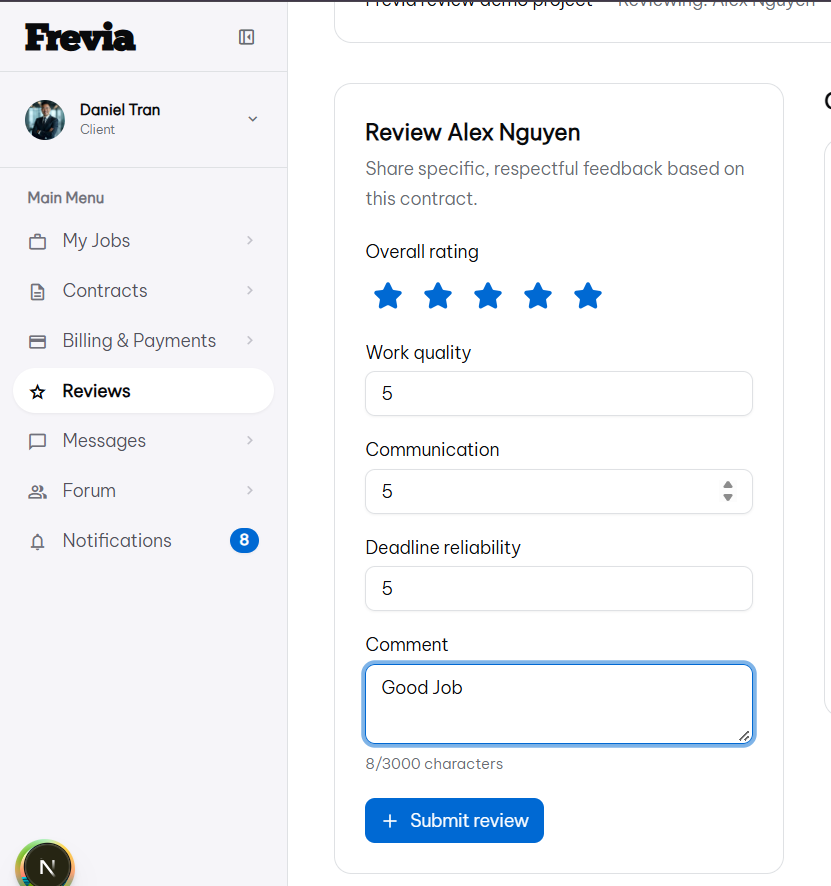
\includegraphics[width=450.00pt]{images/community/m11_05_write_review.png}}
\put(196.65,74.37){\color{fptred}\framebox(216.00,275.87){}}
\put(196.65,350.24){\colorbox{white}{\textcolor{fptred}{\scriptsize\bfseries 1}}}
\put(196.65,21.59){\color{fptred}\framebox(99.90,26.39){}}
\put(196.65,47.98){\colorbox{white}{\textcolor{fptred}{\scriptsize\bfseries 2}}}
\end{picture}
\endgroup}%

\caption{Review form: rating, breakdown, comment and submit action.}
\label{fig:r6_m11_05_write_review}
\end{figure}
\paragraph{Step-by-Step User Instructions:}
\begin{enumerate}[leftmargin=1.8em,itemsep=3pt]
  \item \rbadge{1} Open Reviews and select the relevant completed contract.
  \item \rbadge{2} Choose the overall rating from 1 to 5. Complete Work quality, Communication and Deadline reliability as offered, then enter an optional comment.
  \item \rbadge{3} Select Submit review. To revise your own review, choose Edit, change the fields and save.
  \item \rbadge{4} To remove your own review, select Delete and confirm; select Cancel to keep it.
\end{enumerate}
\paragraph{Expected Output \& Exception Handling:}
\begin{itemize}[leftmargin=1.5em,itemsep=2pt]
  \item \textbf{Expected result:} The selected contract review list reflects a successful creation, update or deletion.
  \item \textbf{Troubleshooting:} You cannot review a different contract's participant or create a second review for the same reviewer/contract. Ineligible contracts and missing permissions do not become eligible by changing the selected rating.
\end{itemize}

\newpage
\subsubsection{M11.06 -- Respond to a Review}
\begin{itemize}[leftmargin=1.5em,itemsep=2pt]
  \item \textbf{Screen Name \& Route Path:}\newline \texttt{/client/reviews or /freelancer/profile?tab=reviews}.
  \item \textbf{Target Actor:} Review recipient.
  \item \textbf{Preconditions:} Signed in; the selected review was addressed to the current user.
  \item \textbf{Purpose:} Publish or maintain a response to received feedback.
\end{itemize}
\paragraph{Screen-Transition Workflow:} Contract review list $\rightarrow$ Respond $\rightarrow$ response editor $\rightarrow$ save, edit or delete.
\begin{figure}[H]\centering
\scalebox{0.75403}{%
\begingroup\setlength{\unitlength}{1pt}\linethickness{0.9pt}
\begin{picture}(450.00,278.50)
\put(0,0){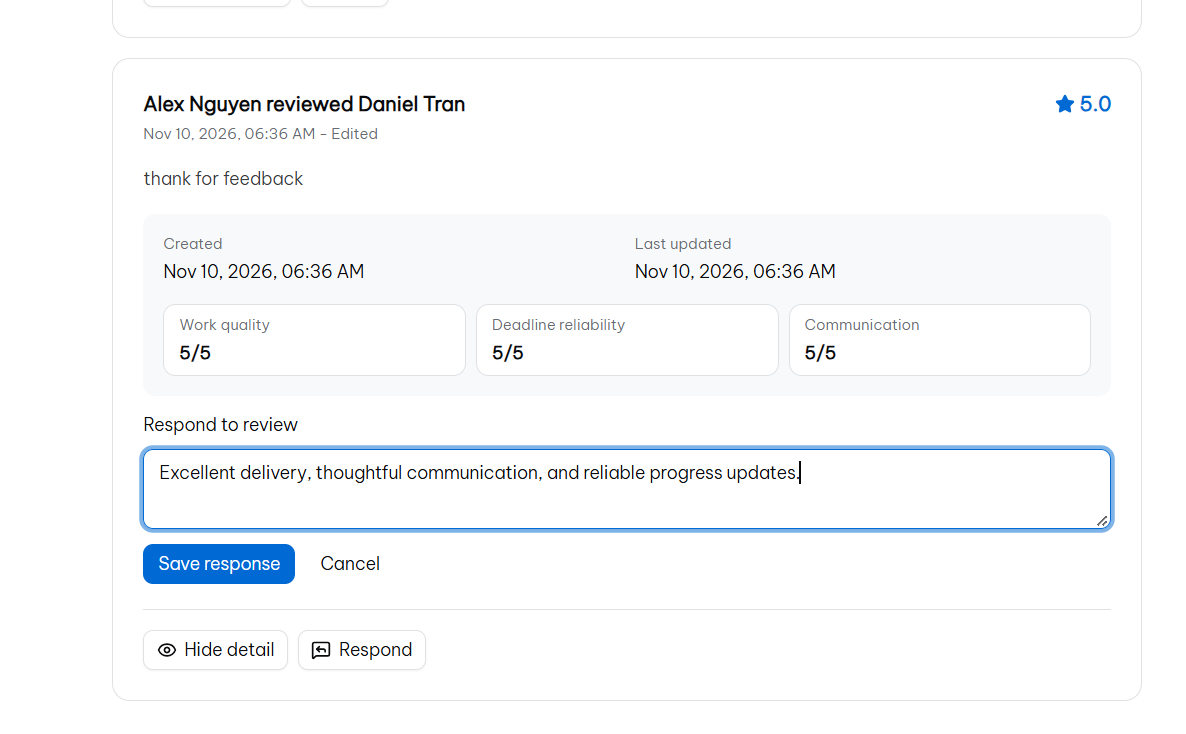
\includegraphics[width=450.00pt]{images/community/m11_06_respond_to_review.png}}
\put(53.55,76.31){\color{fptred}\framebox(368.55,33.14){}}
\put(53.55,109.45){\colorbox{white}{\textcolor{fptred}{\scriptsize\bfseries 1}}}
\put(53.55,56.54){\color{fptred}\framebox(58.50,14.48){}}
\put(53.55,71.02){\colorbox{white}{\textcolor{fptred}{\scriptsize\bfseries 2}}}
\end{picture}
\endgroup}%

\caption{Review response editor and Save response action.}
\label{fig:r6_m11_06_respond_to_review}
\end{figure}
\paragraph{Step-by-Step User Instructions:}
\begin{enumerate}[leftmargin=1.8em,itemsep=3pt]
  \item \rbadge{1} Select the completed contract and locate a review addressed to you.
  \item \rbadge{2} Choose Respond, enter the response text and select Save response; Cancel discards the editor changes.
  \item \rbadge{3} For an existing response owned by you, use Edit to replace its text, or Delete and confirm to remove it.
\end{enumerate}
\paragraph{Expected Output \& Exception Handling:}
\begin{itemize}[leftmargin=1.5em,itemsep=2pt]
  \item \textbf{Expected result:} The saved response appears beneath the corresponding review.
  \item \textbf{Troubleshooting:} Only the review recipient can respond, and only one response is associated with a review. A reviewer does not gain response ownership merely by writing the original review.
\end{itemize}

\newpage
\subsubsection{M15.04 -- Manage Banners}
\begin{itemize}[leftmargin=1.5em,itemsep=2pt]
  \item \textbf{Screen Name \& Route Path:}\newline \texttt{/admin/banners}.
  \item \textbf{Target Actor:} Administrator or authorized internal role.
  \item \textbf{Preconditions:} Signed in with banner-management permissions; image-upload permission is needed to upload an image.
  \item \textbf{Purpose:} Create, inspect, update and delete site banners.
\end{itemize}
\paragraph{Screen-Transition Workflow:} Banners $\rightarrow$ list/search/filter $\rightarrow$ create, details or edit $\rightarrow$ save; delete $\rightarrow$ confirmation.
\begin{figure}[H]\centering
\begin{minipage}[c]{0.48\textwidth}\centering
\scalebox{0.4977}{%
\begingroup\setlength{\unitlength}{1pt}\linethickness{0.9pt}
\begin{picture}(432.00,270.00)
\put(0,0){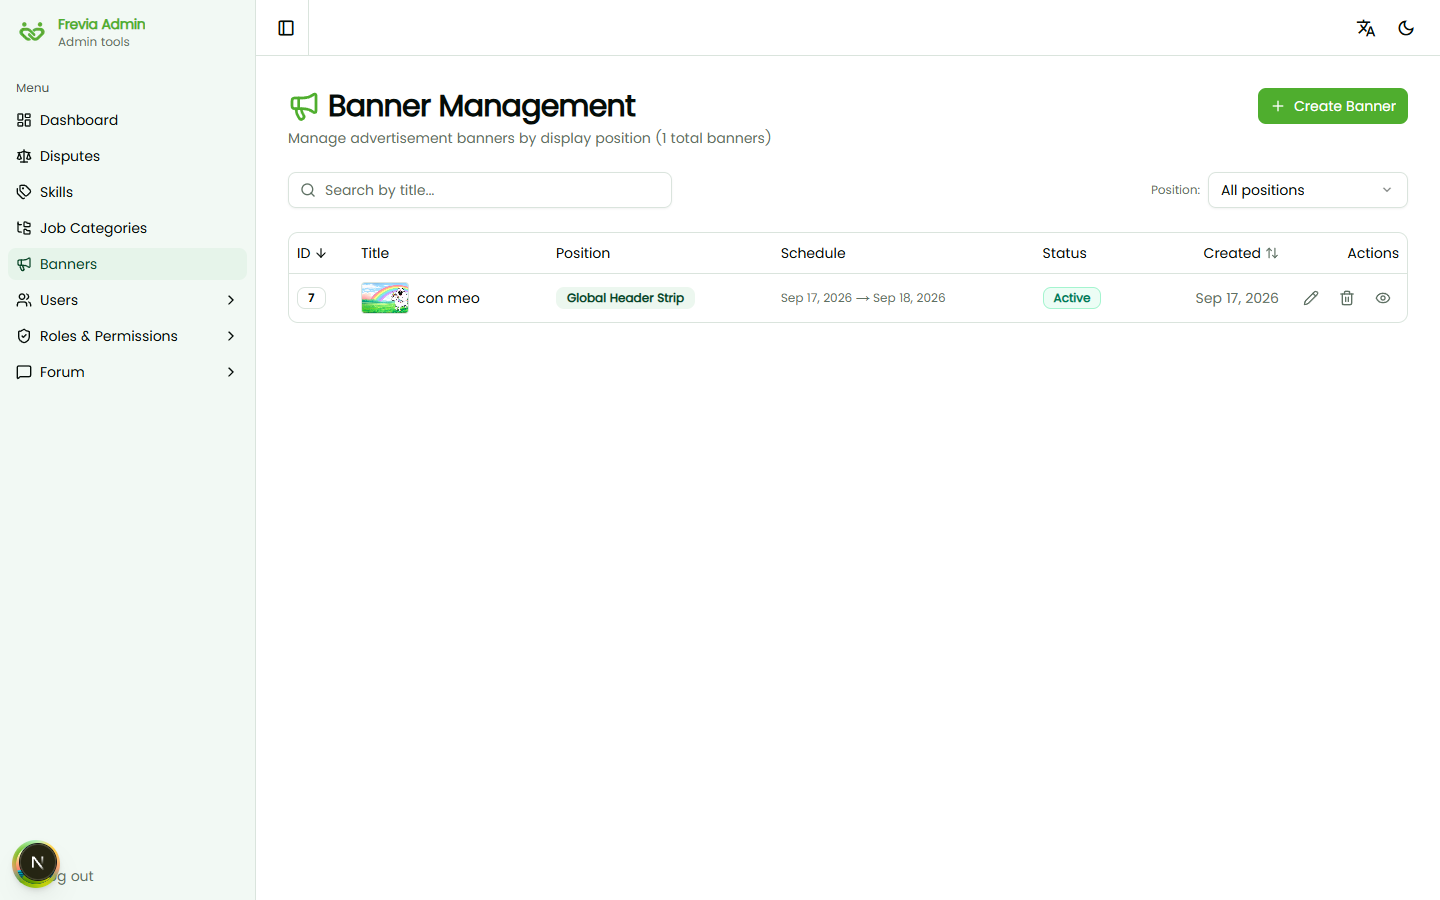
\includegraphics[width=432.00pt]{images/admin/m15_04_viewbannerlist.png}}
\put(376.70,232.20){\color{fptred}\framebox(46.22,11.88){}}
\put(376.70,244.08){\colorbox{white}{\textcolor{fptred}{\scriptsize\bfseries 1}}}
\put(85.97,206.55){\color{fptred}\framebox(336.53,12.15){}}
\put(85.97,218.70){\colorbox{white}{\textcolor{fptred}{\scriptsize\bfseries 2}}}
\end{picture}
\endgroup}%
\end{minipage}\hfill
\begin{minipage}[c]{0.48\textwidth}\centering
\scalebox{0.4977}{%
\begingroup\setlength{\unitlength}{1pt}\linethickness{0.9pt}
\begin{picture}(432.00,270.00)
\put(0,0){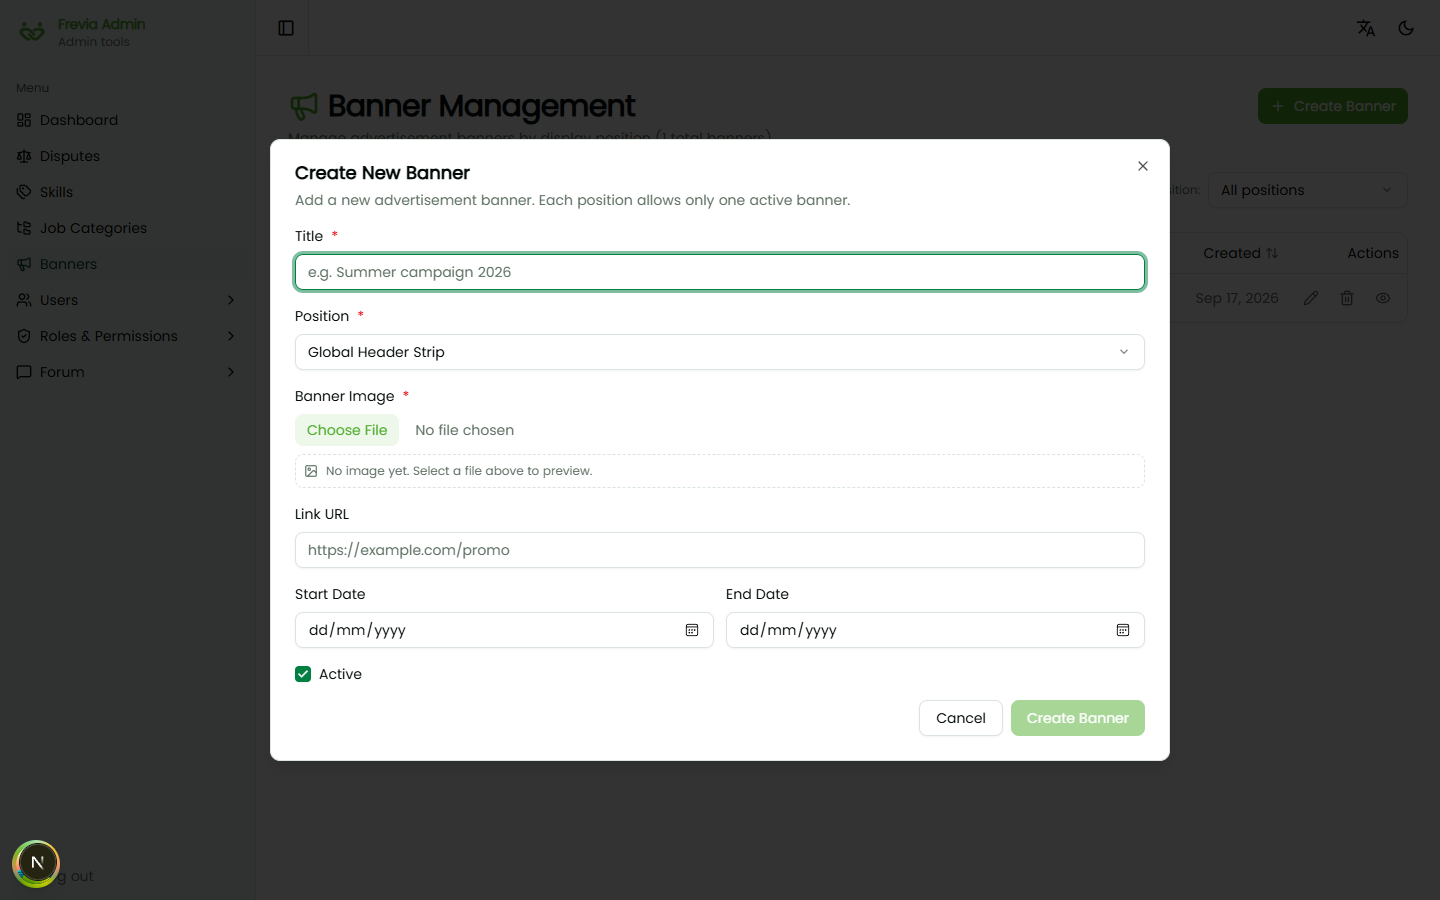
\includegraphics[width=432.00pt]{images/admin/m15_04_createbanner.png}}
\put(87.26,63.72){\color{fptred}\framebox(256.61,137.70){}}
\put(87.26,201.42){\colorbox{white}{\textcolor{fptred}{\scriptsize\bfseries 1}}}
\put(302.40,47.79){\color{fptred}\framebox(41.04,12.15){}}
\put(302.40,59.94){\colorbox{white}{\textcolor{fptred}{\scriptsize\bfseries 2}}}
\end{picture}
\endgroup}%
\end{minipage}
\caption{Banner list, filters and Create Banner action (left); create Banner dialog and form fields.}
\label{fig:r6_m15_04_viewbannerlist}
\label{fig:r6_m15_04_createbanner}
\end{figure}
\paragraph{Step-by-Step User Instructions:}
\begin{enumerate}[leftmargin=1.8em,itemsep=3pt]
  \item \rbadge{1} Open Banners in the Admin Portal. Search by title and use the status/position filters to locate a banner.
  \item \rbadge{2} Select Create Banner. Enter Title, select Position and choose a Banner image. Set the optional Link URL and start/end dates, and select the Active state.
  \item \rbadge{3} Create the banner and inspect its row. Open details to verify the saved image, position, schedule and link.
  \item \rbadge{4} Use the edit action to change the intended fields and Save Changes. To remove a banner, use Delete and confirm Delete banner, or Cancel to keep it.
\end{enumerate}
\paragraph{Expected Output \& Exception Handling:}
\begin{itemize}[leftmargin=1.5em,itemsep=2pt]
  \item \textbf{Expected result:} The list and details reflect successful changes. Visibility depends on the banner's position, schedule and active state.
  \item \textbf{Troubleshooting:} Correct required fields, invalid URLs or inconsistent dates before retrying. If image upload is unavailable, verify upload permission rather than treating a local preview as a successfully uploaded image.
\end{itemize}

\newpage
\subsubsection{M16.01 -- Review Identity Verification Requests}
\begin{itemize}[leftmargin=1.5em,itemsep=2pt]
  \item \textbf{Screen Name \& Route Path:}\newline \texttt{/admin/identity-verifications}.
  \item \textbf{Target Actor:} Administrator or authorized identity reviewer.
  \item \textbf{Preconditions:} Signed in with identity-list, detail and decision permissions as applicable.
  \item \textbf{Purpose:} Inspect submitted identity evidence and record a review decision.
\end{itemize}
\paragraph{Screen-Transition Workflow:} ID Verification Requests $\rightarrow$ search/status tab $\rightarrow$ request details $\rightarrow$ approve or reject $\rightarrow$ refreshed list.
\begin{figure}[H]\centering
\scalebox{0.8254}{%
\begingroup\setlength{\unitlength}{1pt}\linethickness{0.9pt}
\begin{picture}(450.00,254.43)
\put(0,0){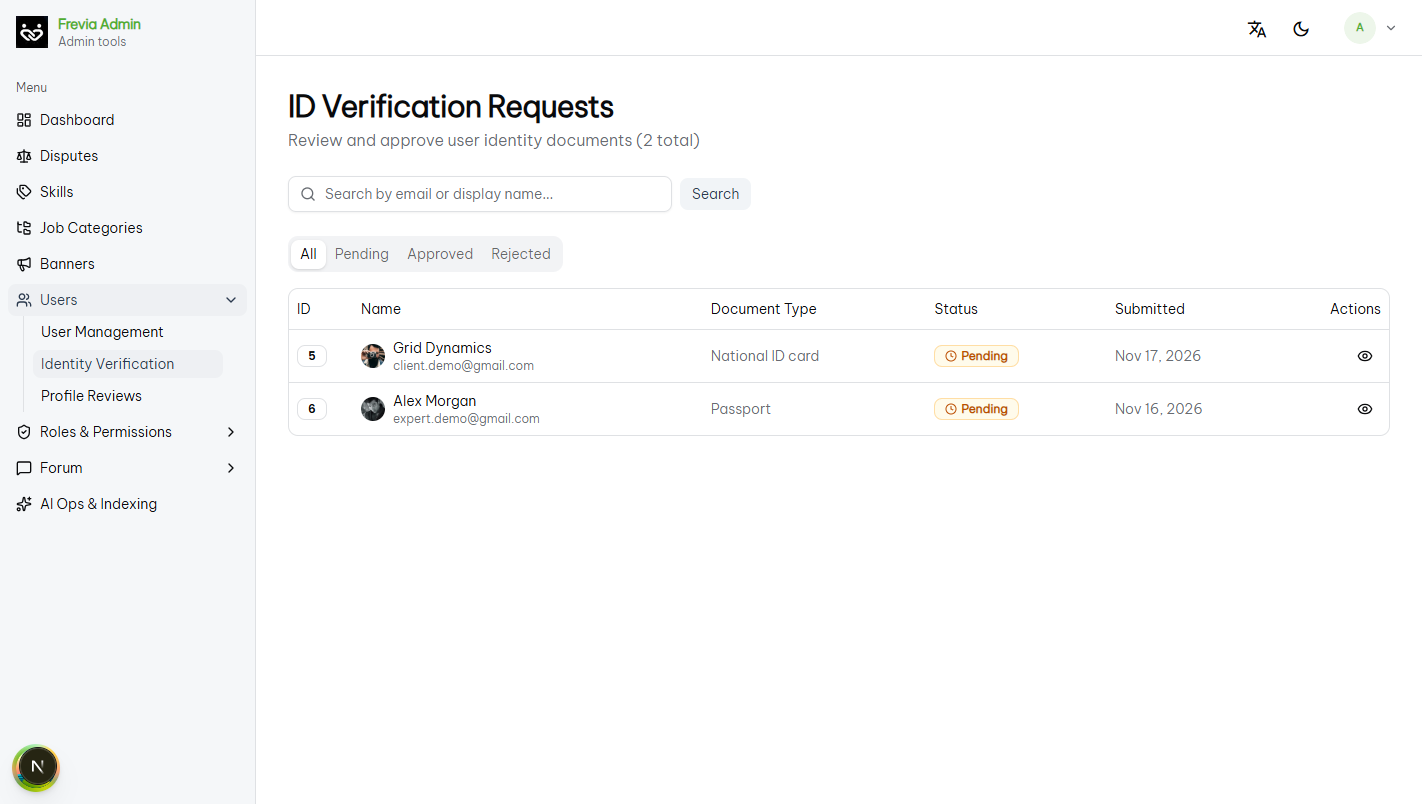
\includegraphics[width=450.00pt]{images/admin/m16_01_adminidentityverifications.png}}
\put(90.00,165.38){\color{fptred}\framebox(153.00,35.62){}}
\put(90.00,201.00){\colorbox{white}{\textcolor{fptred}{\scriptsize\bfseries 1}}}
\put(90.00,115.77){\color{fptred}\framebox(351.00,45.80){}}
\put(90.00,161.56){\colorbox{white}{\textcolor{fptred}{\scriptsize\bfseries 2}}}
\end{picture}
\endgroup}%

\caption{Identity verification queue with search and status tabs.}
\label{fig:r6_m16_01_adminidentityverifications}
\end{figure}
\paragraph{Step-by-Step User Instructions:}
\begin{enumerate}[leftmargin=1.8em,itemsep=3pt]
  \item \rbadge{1} Open ID Verification Requests. Search by email or display name and select Pending, Approved or Rejected as needed.
  \item \rbadge{2} Open a request. Inspect the available document images, selfie/liveness evidence and AI result before deciding.
  \item \rbadge{3} For a Pending record, enter relevant review notes and choose Approve or Reject. Read the confirmation/result and inspect the refreshed status.
\end{enumerate}
\paragraph{Expected Output \& Exception Handling:}
\begin{itemize}[leftmargin=1.5em,itemsep=2pt]
  \item \textbf{Expected result:} The stored verification status and review notes reflect the reviewer's successful decision.
  \item \textbf{Troubleshooting:} Decision controls require their own permissions and a Pending record. If another reviewer has already acted, refresh before making another decision. Do not infer identity approval from an AI pass alone.
\end{itemize}

\newpage
\subsubsection{M16.02 -- Review Profile Update Requests}
\begin{itemize}[leftmargin=1.5em,itemsep=2pt]
  \item \textbf{Screen Name \& Route Path:}\newline \texttt{/admin/profile-revisions}.
  \item \textbf{Target Actor:} Administrator or authorized profile reviewer.
  \item \textbf{Preconditions:} Signed in with revision-list, detail and decision permissions as applicable.
  \item \textbf{Purpose:} Compare published and proposed values before accepting or rejecting a profile revision.
\end{itemize}
\paragraph{Screen-Transition Workflow:} Profile Review Requests $\rightarrow$ search/type/status $\rightarrow$ Review $\rightarrow$ Published/Submitted comparison $\rightarrow$ Approve or Reject.
\begin{figure}[H]\centering
\begin{minipage}[c]{0.48\textwidth}\centering
\scalebox{0.47780}{%
\begingroup\setlength{\unitlength}{1pt}\linethickness{0.9pt}
\begin{picture}(450.00,215.06)
\put(0,0){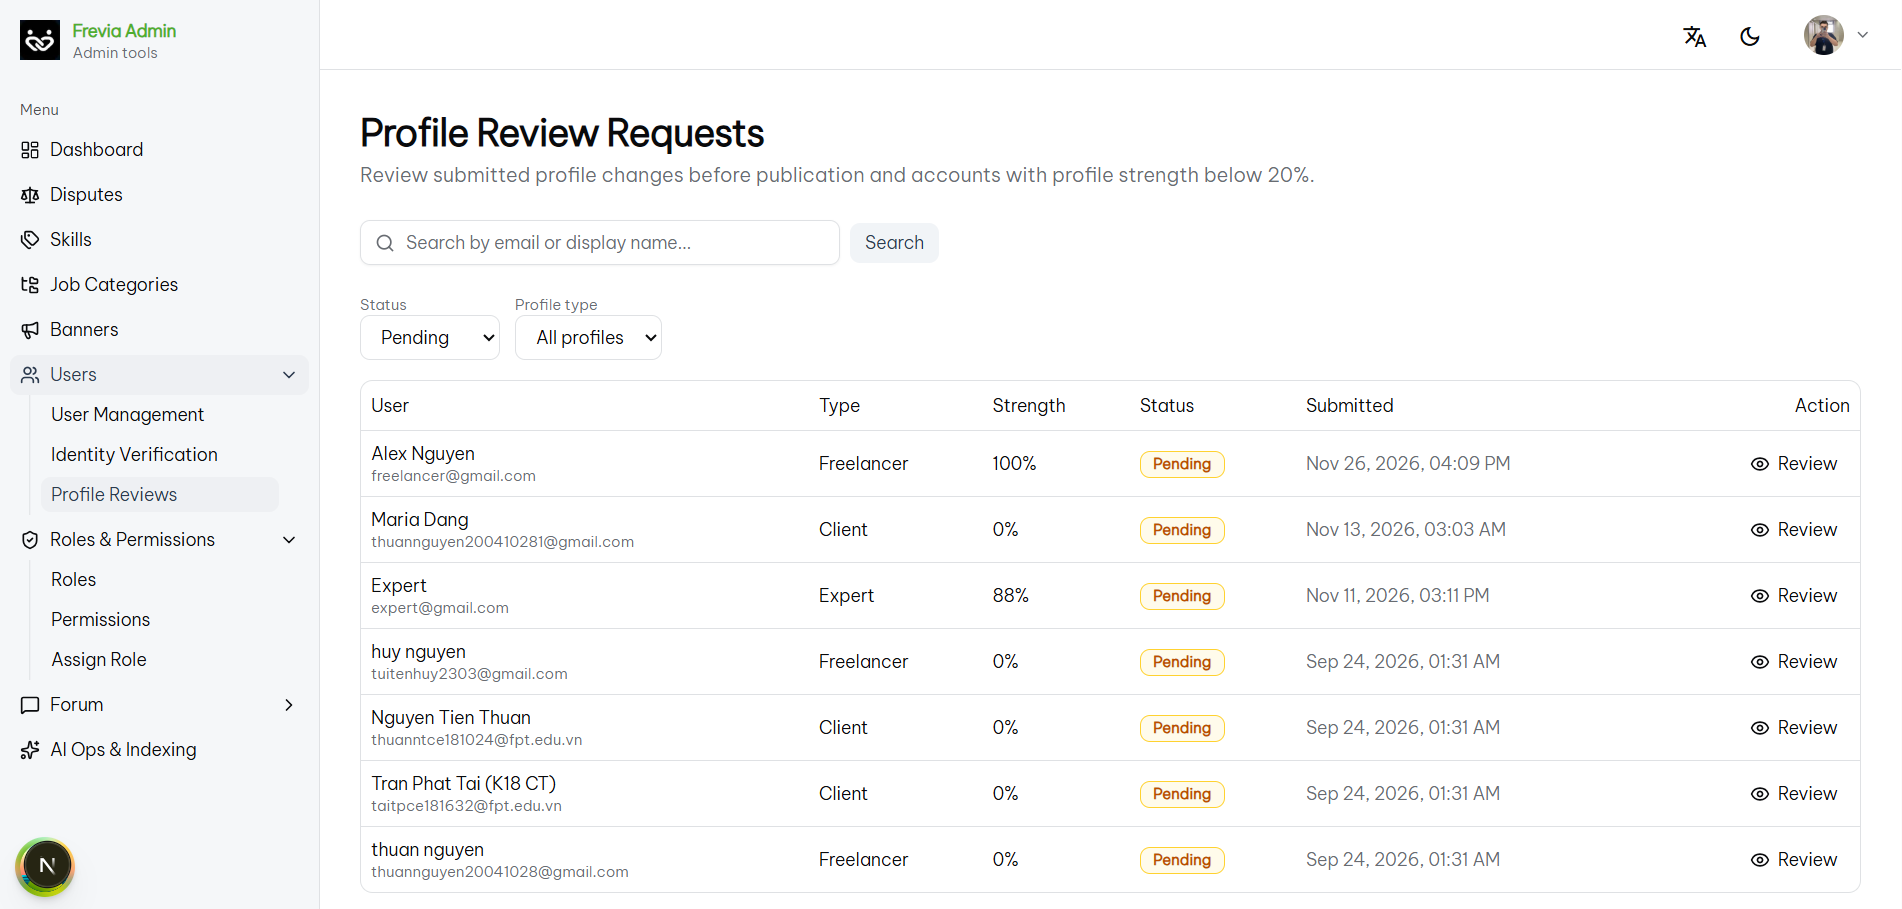
\includegraphics[width=450.00pt]{images/admin/m16_02_view_pending_profile_update_request_list.png}}
\put(83.25,127.96){\color{fptred}\framebox(157.50,36.56){}}
\put(83.25,164.52){\colorbox{white}{\textcolor{fptred}{\scriptsize\bfseries 1}}}
\put(411.75,6.45){\color{fptred}\framebox(29.25,103.23){}}
\put(411.75,109.68){\colorbox{white}{\textcolor{fptred}{\scriptsize\bfseries 2}}}
\end{picture}
\endgroup}%
\end{minipage}\hfill
\begin{minipage}[c]{0.48\textwidth}\centering
\scalebox{0.41246}{%
\begingroup\setlength{\unitlength}{1pt}\linethickness{0.9pt}
\begin{picture}(450.00,213.28)
\put(0,0){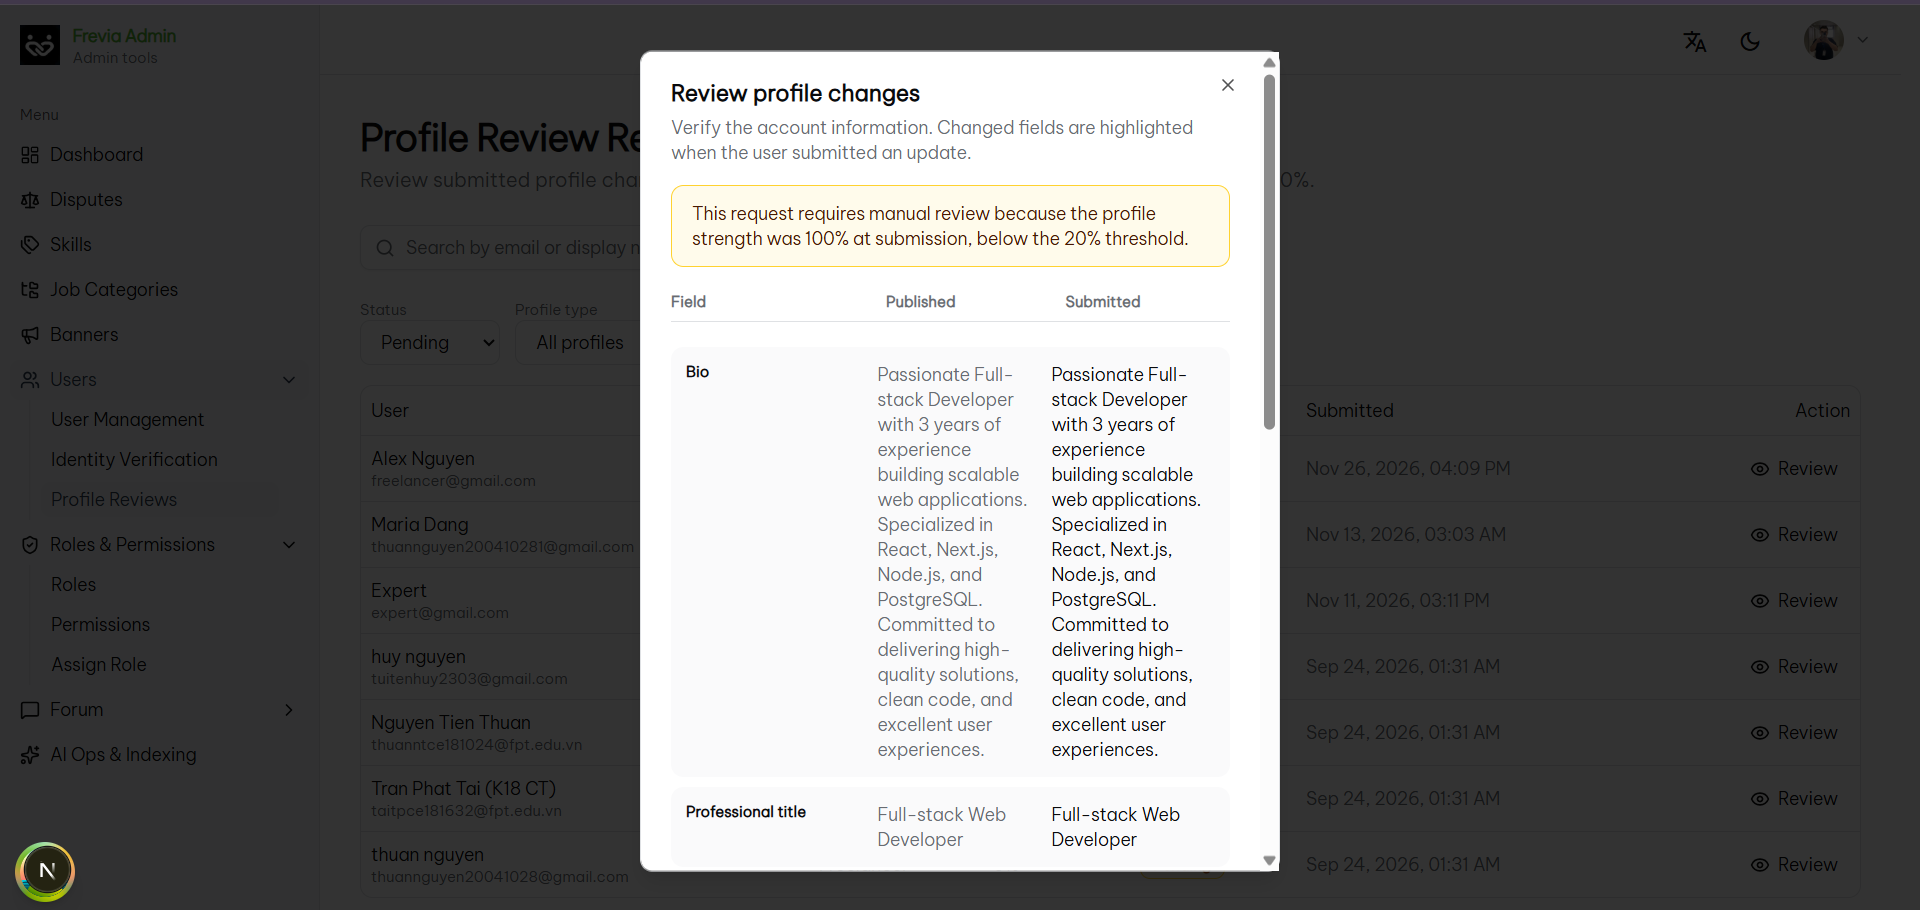
\includegraphics[width=450.00pt]{images/admin/m16_02_view_profile_update_request_detail.png}}
\put(156.60,12.80){\color{fptred}\framebox(132.30,136.50){}}
\put(156.60,149.30){\colorbox{white}{\textcolor{fptred}{\scriptsize\bfseries 1}}}
\end{picture}
\endgroup}%
\end{minipage}
\caption{Profile review queue and Review actions (left); published and Submitted field comparison.}
\label{fig:r6_m16_02_view_pending_profile_update_request_list}
\label{fig:r6_m16_02_view_profile_update_request_detail}
\end{figure}
\paragraph{Step-by-Step User Instructions:}
\begin{enumerate}[leftmargin=1.8em,itemsep=3pt]
  \item \rbadge{1} Open Profile Review Requests. Filter by status/profile type and search by email or display name.
  \item \rbadge{2} Select Review on the intended record. Compare Published and Submitted values field by field; inspect the profile type and strength information.
  \item \rbadge{3} For approval, optionally enter review notes, then select Approve. For rejection, enter a non-empty reason (up to 1000 characters), then select Reject.
  \item \rbadge{4} Refresh the queue and use its status filter to inspect the processed record. Confirm that approval published the intended values.
\end{enumerate}
\paragraph{Expected Output \& Exception Handling:}
\begin{itemize}[leftmargin=1.5em,itemsep=2pt]
  \item \textbf{Expected result:} Approval publishes the accepted revision; rejection retains the published values and stores the reason.
  \item \textbf{Troubleshooting:} Only Pending revisions can be decided. Correct a missing rejection reason. If the record was processed by someone else, reload its current state before continuing.
\end{itemize}
